\documentclass[12pt,a4paper]{article}
\usepackage[left=2.5cm,right=2.5cm,top=2.5cm,bottom=2.5cm]{geometry}
\usepackage[utf8]{inputenc}
\usepackage{amssymb, amsmath, amsthm}
\usepackage{hyperref}
\usepackage{algorithmic, algorithm}
\usepackage{graphics, graphicx}
\graphicspath{ {./7.2/} }

\DeclareMathOperator*{\argmax}{argmax}
\pagestyle{empty}
\hypersetup{
  colorlinks   = true, %Colours links instead of ugly boxes
  urlcolor     = blue, %Colour for external hyperlinks
}

\begin{document}
\textbf{Chapter 7 solutions  \hfill Hanna Gábor}

\begin{enumerate}
  \item
    \textit{In Chapter 6 we noted that the Monte Carlo error can be written as the
    sum of TD errors (6.6) if the value estimates don’t change from step to step. Show that
    the n-step error used in (7.2) can also be written as a sum TD errors (again if the value
    estimates don’t change) generalizing the earlier result.}

    \begin{align*}
      G_{t: t + n} - V(S_t) & = R_{t + 1} + \gamma G_{t + 1: t + n} - V(S_t) + \gamma V(S_{t + 1}) - \gamma V(S_{t + 1})\\
      & = \delta_t + \gamma(G_{t + 1: t + n} - V(S_{t + 1})) \\
      & = \delta_t + \gamma \delta_{t + 1} + \gamma^2 \delta_{t + 2} + \dots + \gamma^{n - 1} \delta_{t + n - 1} + \gamma^{n}V(S_{t + n}) - \gamma^n V(S_{t + n}) \\
      & = \sum\limits_{k = t}^{t + n - 1} \gamma^{k - t} \delta_k
    \end{align*}

  \item
    \textit{Programming. With an n-step method, the value estimates do change from
    step to step, so an algorithm that used the sum of TD errors (see previous exercise) in
    place of the error in (7.2) would actually be a slightly different algorithm. Would it be a
    better algorithm or a worse one? Devise and program a small experiment to answer this
    question empirically.}

    There is only a difference in the two methods if we update state estimes for some states from
    $\{S_{t + 1}, \dots S_{t + n}\}$ between time steps $t$ and $t + n$. Because of this reason,
    I would like to try the algorithms on a problem where we may return to the same
    state shortly. My expectation is that the $n$-step update works better, because it uses
    a more recent estimation of $V(S_t)$. It does not use estimations of $V_(S_{t + i})$
    (for $i = 1 \dots < n$) either, but I am not sure if it is for the better or the worse. Let's try it on a random walk example, like in Example 6.2.

    The code can be found at \url{https://github.com/hannagabor/SBRL/blob/master/7.2/random_walks_td.ipynb}.

    The results show that if alpha is bigger, then the TD-error update is worse than the original n-step method. If alpha is small enough, then there is no
    difference. (At least on this problem.)
    \begin{center}
    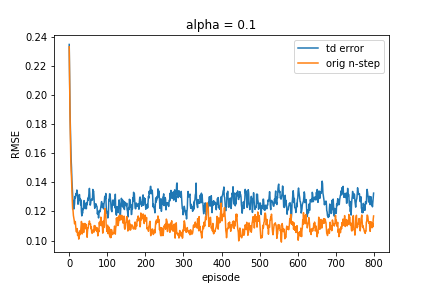
\includegraphics[scale=0.45]{0.1}
    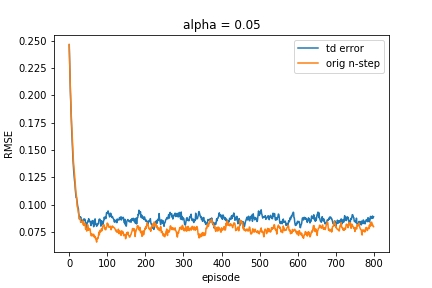
\includegraphics[scale=0.45]{0.05}
    \\
    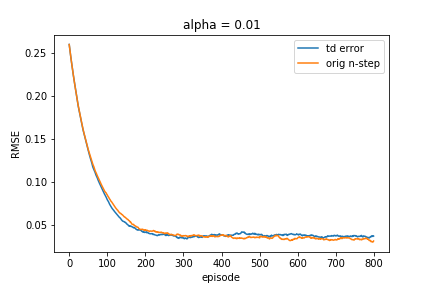
\includegraphics[scale=0.45]{0.01}
    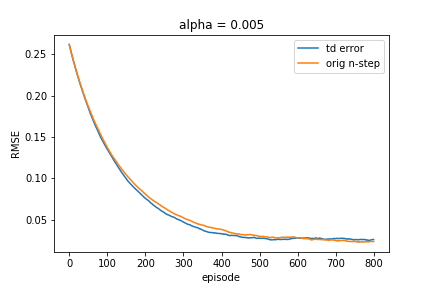
\includegraphics[scale=0.45]{0.005}
    \end{center}


\end{enumerate}
\end{document}
